\documentclass[12pt]{article}

\usepackage{fullpage}
\usepackage{graphicx, rotating, booktabs} 
\usepackage{times} 
\usepackage{fbb} 
\usepackage{natbib} 
\usepackage{indentfirst} 
\usepackage{setspace}
\usepackage{grffile} 
\usepackage{hyperref}
\usepackage{tikz}
\usepackage[export]{adjustbox}
\usepackage[most]{tcolorbox}
\usepackage{verbatimbox}
\usepackage{lscape}
\usepackage{afterpage}
\usepackage{amsmath}
\usepackage[labelfont={bf},textfont=it,labelsep=period]{caption}
 \usepackage{multirow} 
\setcitestyle{aysep{}}
\usepackage{dcolumn}

\hypersetup{
  colorlinks = true,
  urlcolor = blue,
  linkcolor = black,
  citecolor = black,
  pdfauthor = {Joshua Alley},
  pdfkeywords = {},
  pdftitle = {},
  pdfsubject = {},
  pdfpagemode = UseNone,
%  pdffitwindow = true
%  pdfcenterwindow = true
}



\singlespace
\title{\textbf{Economic Bargaining in Asymmetric Alliances}}
\author{
Joshua Alley\\
Postdoctoral Research Associate\\
Democratic Statecraft Lab\\
University of Virginia 
}
 
\date{\today}

\bibliographystyle{apsr}

\usepackage{sectsty}
\sectionfont{\Large}
\subsectionfont{\noindent\large\textit}
\subsubsectionfont{\normalsize}

\makeatletter
\renewcommand\tiny{\@setfontsize\tiny{9}{10}}
\makeatother


\begin{document}

\maketitle 

\begin{abstract}
Can military alliance leaders leverage their preponderant security role to extract economic concessions from junior partners?
Some argue that powerful states can manipulate their security commitments to coerce economic changes. 
Others believe that large states value security ties too much to exert economic leverage.  
I argue that large states usually have limited alliance leverage, but junior alliance members will make temporary economic concessions to support committed allied leaders' tenure in office.
When a patron state leader has signaled substantial alliance commitment, alliance proteges help them boost the economy during leadership competitions.  
I test these claims with analyses of U.S. trade with allied states. 
I find that prior leader signals of commitment increase exports to allied states during election years. 
A subsequent examination of election-year exports from U.S. states shows that increased trade with allies concentrates in swing states. 
Finally, I find that these trade concessions are temporary, as allies do not adjust their tariff policies in response to changing leader commitment or electoral cycles. 
These results suggest that leaders can employ security commitment for temporary economic and political gain as allies facilitate political business cycles. 
\end{abstract} 


\newpage 
\doublespace 


\section{Introduction}

%In 2018, a former Obama administration official argued that ``"Trump is trying to conflate his issues over trade and his beef with Europe and the EU with NATO, and he's using our military strength to do that.''\footnote{\url{https://www.usatoday.com/story/news/politics/2018/07/11/donald-trump-complains-trade-europe-nato-summit/774495002/}}
In 2019, when Donald Trump argued that ``It's not right to be taken advantage of on NATO and also then to be taken advantage of on trade, and that's what happens,'' he was not the first or last U.S. policymaker to highlight perceived problematic economic concessions to allies.
Then Secretary of the Treasury John Connally claimed in a 1971 speech that the United States ``had the right to expect more equitable trading arrangements'' with its allies (quoted in \citet[pg 175]{Sayle2019}).
%\footnote{See also: \url{https://www.fpri.org/article/2019/04/the-blue-chip-and-the-little-blue-bird-change-and-continuity-in-nato-policy-from-nixon-to-trump/} and \url{https://history.state.gov/historicaldocuments/frus1969-76v03/d155}}
More recently, some leading congressmen criticized the Biden administration's decision to waive sanctions on the Nord Stream 2 gas pipeline between Russia and Germany.\footnote{\url{https://www.bbc.com/news/world-us-canada-57180674}}


These examples reflect a general question; can large alliance leaders like the United States leverage their preponderant security role for economic influence over junior allies? 
There are two schools of thought on economic bargaining in asymmetric alliances. 
One argues that because leading states prioritize geopolitical aims, they have limited economic leverage \citep{Drezner2013, WolfordKim2017}.
Another perspective argues that threatening to reduce security commitments encourages economic concessions \citep[pg. 122]{Oatley2015}. 


I argue that large alliance members' economic leverage depends on potential leadership changes and past efforts to reassure allies.
When leaders establish a reputation for alliance commitment, they usually reduce their leverage over allied economic policies. 
A prior reputation for commitment increases leverage when leaders seek economic concessions to support their efforts to remain in office. 
Small allies will make economic concessions if they help a committed partner retain power without endangering their own tenure in office.  
Thus, leaders who have previously demonstrated commitment to an alliance are more likely to secure economic concessions, but those concessions will be temporary and targeted, rather than structural.
Trade with allies will increase around election years for committed leaders and concentrate in key electoral constituencies. 
At the same time, prior commitments and election timing will have no impact of tariffs, as these structural concessions endanger allied leaders' domestic political survival. 
Senior allies thus have little economic leverage, unless potential leadership change encourages their partners to make economic concessions to bolster their long-run security. 


% Findings
I test the argument in three ways.
First, I analyze U.S. exports to allied countries because fixed U.S. elections provide clear indications of potential leadership change and the United States has a significant role in many asymmetric alliances. 
I find that when U.S. leaders signal more support to allied states, those states increase imports from the United States as proximity to an election year approaches. 
Leader signals of support decrease U.S. exports in more distant years, however. 
A subsequent analysis of exports from U.S. states in election years suggests that allies concentrate their imports in electorally competitive states, which is consistent with strategic imports to impact electoral competition.
The final analysis shows that unlike trade flows, prior leader commitment and elections have a negligible association with allied tariffs on U.S. goods. 


% economic and seucrity ties 
The argument and findings address three salient issues in international relations theory and practice. 
First, they speak to debates about the connection between economic and security ties \citep{Mastanduno2009, Poast2019}. 
Scholars dispute whether economic linkages drive security ties \citep{BiglaiserDeRouen2007, Fordham2010, Kimball2010}, security concerns encourage economic linkages \citep{Gowa1995, Li2003, LongLeeds2006, GowaMansfield2004}, or the relationship goes in both directions \citep{BiglaiserDeRouen2009, KinneBunte2018}. 
My findings suggest that the direction of the relationship depends on electoral cycles. 
Security concerns shape economic links in most years, but the relationship flips when states use economic policies to cement security relationships.


% economic cycles
Expanded exports from alliance leaders to junior partners in election years also reflect political business cycles where elites manipulate economic policy to win reelection. 
Elected leaders often use fiscal \citep{Rogoff1987} and monetary policy \citep{ClarkHallerberg2000} to generate economic growth around elections. 
There is also evidence that leaders use non-budget instruments like social policy \citep{Philips2020}, social pacts with unions \citep{Ahlquist2010}, trade disputes \citep{Conconietal2017} and defense contracts \citep{DerouenHeo2000} to bolster their electoral prospects. 
I find that allies expand trade and contribute to political business cycles when the incumbent leader supported their security interests.


% coercion
Finally, this paper provides new insight into coercive demands by bridging economic and security bargaining.
When and why coercion succeeds is a salient question (e.g \citep{Sechser2010, Sechser2018, Cebuletal2021}).  
Most studies of coercion examine either security threats (e.g. \citep{HorowitzReiter2001, Sechser2011}) or economic sanctions (e.g. \citep{Marinov2005, Allen2008, Escriba-FolchWright2010}).
This study explores whether security ties provide economic leverage. 
In particular, it explores issue linkage as part of alliance management, building on previous work that considers alliance formation \citep{Poast2012} and credibility \citep{Davis2008, Poast2013}. 


% policy 
Whether trade concessions are the price of security alliances also has important implications for how policymakers bargain with allies. 
If threats to reduce security commitments do not lead to economic concessions, then they create negative security consequences without corresponding economic gains for either party. 
But a cooperative equilibrium where leaders signal support for allies and allies support their tenure in office is possible. 



% need an outline 
The paper proceeds as follows. 
To start, I outline an argument explaining when and why alliance leaders might demand economic concessions from their partners, and when allies might offer economic assistance. 
I then test three predictions from the argument. 
First, I show that U.S. exports and trade with allies increases more in election years as prior leader signals of support increase. 
I then show that expanded election year trade between the U.S. and its allies is concentrated in swing states. 
Finally, I examine tariff levels and show that allies are unlikely to make structural concessions, even as commitment signals increase. 


\section{Argument}


%Whether large alliance members can coerce economic change in smaller allies also adds a new dimension to our understanding of coercion. 
%Classic studies of coercion with security threats often focus on security outcomes in a crisis bargaining framework \citep{Sechser2011, Cebuletal2021}. 
%Other studies of economic coercion through sanctions considers political \citep{Marinov2005, Bapatetal2016} and economic aims. 
%This study examines how security threats shape economic ties. 
%Prior scholarship on gunboat diplomacy and trade is the most closely related work in prior scholarship. 
%\autoref{tab:sec-econ-coerce} summarizes the place of this work in studies of coercion.
%
%
%
%\begin{table}[hbt!]
%\begin{center}
%\begin{tabular}{| p{0.2\linewidth} | p{0.4\linewidth} | p{0.4\linewidth} | }
%\hline
%              &   Security Threat & Economic Threat \\
%\hline                  
%Security Demand  & Crisis Bargaining &  Sanctions for Political Change \\
%Economic Demand  & \textbf{Economic Bargaining Between Allies}, Gunboat Diplomacy  &  Sanctions for Political Change  \\     
%\hline                          
%\end{tabular}
%\caption{Potential threats and aims in coercive bargaining.}
%\label{tab:sec-econ-coerce}
%\end{center} 
%\end{table}


% basic asymm alliance framework
This argument addresses economic bargaining in asymmetric alliances. 
In alliances between large and small states, the large state protects its junior partner in exchange for foreign policy concessions \citep{Morrow1991}.
By providing costly and credible military support commitments, the large state increases their foreign policy influence. 
Small alliance members garner protection from external threats and the cost of foreign policy autonomy. 


Military alliances are inseparable from economic cooperation.
Conflict and economic integration are linked in general (see for example, \citep{GartzkeLi2003, Chen2021}).
Many alliances also include explicit or implicit linkages to economic cooperation \citep{GowaMansfield2004, LongLeeds2006, Davis2008, Poast2012}. 
Thus alliances often reflect a cooperative bundle of security and economic ties. 


There are two competing perspectives on the balance of security and economic relations in asymmetric alliances.
Although many asymmetric alliance reflect a hierarchical relationships, security and economic hierarchy are not equivalent \citep{Lake2009}. 
One argues that to prioritize international influence and geopolitical concerns, large state leaders tolerate economic protectionism \citep{Drezner2013, WolfordKim2017}. 
In this perspective, large state leaders prioritize security over economic influence, leaving little economic leverage. 
Another view claims that threats to reduce commitment can coerce economic concessions from junior alliance partners \citep{Oatley2015}.  


% overview
I argue that large alliance members usually lack economic leverage, especially when they invest in credible alliance commitments, but when a committed leader might be replaced, allies will make economic concessions. 
The relationship between alliances and economic bargaining thus depends on leader investment in alliance commitment and leadership competition in the large alliance partner.  
Only leaders with an established reputation for cooperation with allies can leverage their security commitments for economic concessions, and then only around elections. 
Allies will make temporary concessions to support a friendly leader without endangering their own security in office. 
This process thus highlights the role of leaders in intra-alliance bargaining. 


% actors 
There are four key actors in this argument. 
First, the large alliance member leader seeks geopolitical influence and a favorable balance of economic relations. 
Second, a leader in the small alliance member seeks security from external threat and a favorable economic balance.
Both leaders are office-seeking and depend on domestic supporters to stay in power.
The third and fourth actors are are domestic actors in both states can gain or lose from changes in economic ties between the allied states. 


% issue- must keep domestic actors happy to retain power
Leaders require domestic support to win and continue in office.
Trade policy shapes domestic policies, as trade barriers have distributional consequences for domestic interests in large and small alliance members.
Under incomplete trade openness, some domestic sectors in both states are protected from foreign trade competition by tariff or non-tariff barriers. 
Protected sectors have higher incomes than they would under free trade, while sectors with a comparative advantage in the other state lose out on gains from trade. 


Junior alliance members have strong incentives to protect domestic interests from trade with a patron state. 
Large alliance leaders often have market power in international trade. 
Keeping out exports increases the income of protected sectors in the junior alliance member that would otherwise have to compete with exports from the large state.
Concessions to a large ally would reduce their income and support for the incumbent leader, as trade cleavages shape domestic political coalitions \citep{Rogowski1987, Hiscox2001}. 


% response: lean on allies for concessions, especially when there's a risk of losing office
Given junior partners' trade protection, there are two domestic political motives for large state leaders to renegotiate the balance of economic and security relations in an alliance. 
First, trade liberalization could benefit large allied exporters by increasing their market share.
Increased exports to junior members could benefit domestic interests, who would then reward the incumbent with political support. 
Second, expanded trade could increase domestic consumption, which voters can reward. 


%  
Large state leaders can benefit from changing the economic bargain in an alliance throughout their tenure, but the benefits are crucial when they risk losing office through an election or some other leadership challenge. 
Leadership competition increases the pressure on leaders to solidify their existing coalition or find new supports. 
Even as leaders face term limits, they will often seek to ensure that their coalition remains in power. 


% exact threat 
When leaders want to increase trade, alliance security guarantees are a plausible source of economic leverage. 
If the initial alliance contained an implicit or explicit economic arrangement, those bargains can be renegotiated during alliance maintenance. 
Threatening to reconsider their security commitments to smaller partners might increase large state leaders' economic influence. 
Leadership competition motivates using security threats for economic gains, as allied economic policies affect prosperity and leadership competition. 


% making the threat credible
Credible threats to reduce security commitments in exchange for economic concessions depend on prior investment in the alliance, however. 
If a leader has not invested in the alliance, their allies have less security to preserve by helping them remain in office. 
And if there is no risk of leader turnover, allies need not account for the danger that changes in the ruling coalition will reduce their security from the alliance. 
Given leadership competition, economic demands contain an implicit threat that failing to concede might endanger security cooperation by empowering a less committed leader.


% allied incentives to concede- want to keep security, must keep their interests happy too
% new leader might be similar, but less certainty. 
Security threats in economic bargaining can create a dilemma for small alliance members. 
Reduced alliance commitments endanger small state security, but economic concessions threaten a leader's hold on office by harming domestic interests. 
Small state leaders thus weigh the likely security benefits of conceding against the domestic political economy consequences.


% security benefits- leader coop
The security benefits of conceding to a patron state leader depend on that leader's prior commitment to the alliance. 
In economic bargaining between allies, reputations for commitment adhere to leaders, who have substantial influence on foreign and economic policy \citep{Renshonetal2018}.
Executive leaders have a crucial role in alliance politics, as they have a pivotal role in decisions to use force (e.g \citep{Colgan2013, ColganWeeks2015}).
Just as leadership changes can increase the risk of international crisis \citep{Wolford2007}, a leader's reputation for alliance cooperation shape how allies respond to their economic demands. 


Leaders establish alliance commitment by tying their hands and sinking costs \citep{Fearon1997}. 
Statements of reassurance and commitment to an alliance are one salient way for leaders to establish a cooperative reputation \citep{Blankenship2020}.
Leaders can also deploy troops, visit allied states, offer aid, and employ other sunk cost signals of support \citep{McManusNieman2019}.
Both these efforts indicate that a leader is willing to honor their alliance commitments. 


% need to establish commitment early
If leaders are committed to an alliance, establishing credibility early in their tenure is crucial. 
New leaders' alliance commitment is private information to allies and adversaries. 
Taking costly actions shows whether a leader is committed to the alliance in the same way that new leaders establish a reputation for resolve in crisis bargaining \citep{Wolford2007}. 


% only concede if enough prior res: cooperative reputation
Small alliance member leaders will only make economic concessions if they believe that supporting the efforts of the large alliance leader to retain power offers sufficient security benefits. 
Economic concessions thus depend on the large state leader's cooperative reputation. 
If the large state leader has demonstrated strong commitment to the alliance before making economic demands, then adjusting economic relations to help them retain power is worthwhile.
Small state leaders prefer a cooperative partner to an uncertain leadership change, given the high stakes of changes in alliance commitments.
If a leader has not tied hands or sunk costs, then allies may be willing to gamble on the next leader being more invested. 
At a minimum, allied states have few incentives to aid a leader who has not invested in their security. 


% prior res establishes rep for restraint too: cebul et al
In addition to establishing that concessions will bolster protege security by helping a friendly leader remain in office, prior cooperation generates a necessary reputation for restraint. 
Committing to not renege and follow through on a threat regardless of cooperation is essential in coercive bargaining \citep{Cebuletal2021}. 
If a leader previously demonstrated commitment to the alliance, it reduces the perceived risk that they will demand further concessions, or reduce security commitment regardless.
This decreases the likelihood of proteges rejecting economic demands to establish a reputation for resolve to ward off future challenges \citep{Sechser2010, Sechser2018}. 


% prior commitment helps in three ways
Prior commitment provides conditional and limited economic leverage. 
Some concern with leadership change is necessary for commitment to increase patron influence. 
Allies will also make temporary changes, rather than adjusting tariff schedules or making other structural shifts. 
Those changes will be targeted to maximize their influence on leadership competition, however. 


% early comm, reduced leverage
Prior commitment signals increase leaders' economic influence when they might be replaced, but reduce it otherwise. 
Investing in security for junior allies makes threats to renegotiate the balance of security and economic relations less credible. 
Moreover, when leaders can provide another commitment signal by showing their support and then tolerate the resulting economic protectionism by allies. 
Bearing the costs of allied economic actions is a costly signal of commitment to an alliance because it generates economic inefficiencies. 
It also changes the domestic politics of the protege in favorable ways for the patron \citep{Lake2013}. 


% don't concede too much, however
Even when a leader creates a cooperative reputation and faces replacement, domestic concerns constrain allied economic concessions \citep{Davis2008}. 
Reducing protection for domestic industries exposes a leader to domestic political pressure. 
Taking down trade barriers is also hard to reverse, especially when states are part of international organizations.
Structural changes increase the risk of a small state leader losing office.  
The result is that small states will make temporary concessions to help cooperative leaders remain in office, while avoiding structural changes. 
Symbolic, temporary and targeted measures can give a large state incumbent a competitive boost without antagonizing domestic interests. 
Large states can therefore only leverage security preponderance security role at specific times and in limited ways.


% Govt purchases to address BoP and trade deficit. 
Although small states do not make structural concessions, they do make targeted changes that maximize their influence on leadership competition.
Government purchases provide a way to undertake targeted changes in trade policy with reducing protection for domestic interests. 
For example, \citep{Bergeretal2013} find that CIA interventions increased U.S. exports to targeted countries via government purchases.


% Might even be targeted by region. 
Small states can impact leadership competition in the large state by focusing their economic efforts on key constituencies.
Proteges could target their purchases in crucial electoral districts to bolster a cooperative democratic leader, for instance. 
In autocracies, purchases could favor members of the leaders' winning coalition, whether by geography or sector.


% explains a couple recent things- illustrative
% why'd Biden concede on Nord stream 2? 
Several recent interactions between the United States and its allies help illustrate the argument. 
First, the Biden administration's controversial decision to waive sanctions and allow completion of the Nord Stream 2 gas pipeline between Germany and Russia is likely part of the Biden administration's efforts to reassure European allies. 
In addition to allowing this concession to German economic concerns, Biden sought to wind down many of Trump's European trade disputes while talking up the U.S. commitment to NATO and the EU.\footnote{\url{https://www.aljazeera.com/economy/2021/6/15/eu-and-us-call-truce-in-trump-era-trade-war}}


% why did Trump fail to get substantial economic concessions from allies? 
The argument also explains why U.S. allies rarely conceded Donald Trump's trade demands. 
Trump's prior rhetorical attacks on NATO and other U.S. alliances gave allies few incentives help him win re-election. 
Economic concessions might have aided Trump's re-election campaign, just as Chinese tariffs on soy reduced Republican's vote share in the 2018 election \citep{ChyzhUrbatsch2021}. 
Moreover, Trump sought fundamental alterations to trade policy such as reduced barriers to U.S. agricultural products that might have endangered allied leaders' political survival \citep{HeeParkJensen2007}.



\subsection{Implications}



In addition to the suggestive evidence from these U.S. examples, the argument has several testable implications, especially for democratic alliance leaders.
Elections provide clear indicators of when a leader might be replaced. 
This also facilitates strategic anticipation on the part of allies and leaders, who can adjust their economic bargaining accordingly. 
The relatively open nature of electoral competition also facilitates allied influence from economic concessions. 


The first hypothesis concerns when and how junior partners make economic concessions. 
Junior partners will increase their imports from allies when the leader facing replacement has demonstrated prior commitment to the alliance. 
Otherwise, junior alliance members may take a chance on elections empowering a more supportive leader. 
Past indicators of commitment include statements of reassurance \citep{Blankenship2020} and trade concessions \citep{WolfordKim2017}.


\begin{quote}
\textsc{Economic Concession Hypothesis: When the leader of a large alliance member might be replaced, the trade balance with junior allies will increase as prior commitment signals by that leader increase.}
\end{quote}



The second hypothesis predicts targeted concessions.
If allies want to support a friendly leader, they may target their economic concessions to crucial regions of electoral contests. 
In the United States, swing states have a critical role in presidential elections, which encourages U.S. leaders to focus on them in economic policies like WTO disputes \citep{Conconietal2017}.
Therefore, one potential implication is that exports from swing states to U.S. allies will increase in the year of elections more than exports from other states.

\begin{quote}
\textsc{Swing States Hypothesis: During presidential election years, exports from states to U.S. allies will be increase as electoral competition in that state increases.}
\end{quote}

%
%The third prediction is that economic pressure from larger allies will be more likely when the leader faces replacement through election or some other competition. 
%Given pressure to deliver for domestic interests to remain in office, leaders will be more likely to make economic demands of allies when there is a high chance they will be replaced. 
%These demands are especially likely to cover issues with distributional consequences like trade.
%
%
%\begin{quote}
%\textsc{Economic Demands Hypothesis: As the likelihood of a leadership change increases, leaders of large alliance members will make more economic demands of allies.}
%\end{quote}


The third prediction is that junior allies are unlikely to make tariff concessions. 
Although helping a committed leader remain in office is valuable, the leaders of junior alliance members cannot endanger their own tenure by antagonizing domestic interests.
Therefore, even if a large state leader has offered substantial commitment and faces electoral replacement, their reassurances will be unlikely to alter allied tariff schedules. 


\begin{quote}
\textsc{Tariff Hypothesis:  When the leader of a large alliance member might be replaced, tariffs by junior allies, even as prior commitment signals by that leader increase, tariff levels will undergo negligible changes. }
\end{quote}



\subsection{Objections and Alternative Explanations}


% objection- why not dismiss threats/demands by committed leaders as incredible? 
% stand to benefit from helping them
Before proceeding to how I test these hypotheses, I consider several potential objections and alternatives to the argument, including whether committed leaders can make credible economic demands and the role of external threat.
First, why do junior partners to concede economic demands to committed leaders? 
While government purchases are less consequential than tariff changes, spending funds on U.S. exports still imposes opportunity costs.
I expect that purchases are worthwhile to support the security benefits of a committed allied leader. 
Conceding purchases greater security in expectation. 


% threat: increases sec demand, but makes it harder to walk away for large partner
% Cold War should make that fairly clear. 
Another objection is that increased external threat might make junior alliance partners more receptive to economic demands from their patron.
Conceding to ensure protection might be worthwhile, in short.
Though this is plausible, it ignores the incentives of the large partner, who also has more to lose from weakening an alliance if the threat to junior partners is greater. 
Cold War dynamics illustrate this issue.
Although the United States initially tolerated and even encouraged European and Japanese protectionism to ensure that allies could rebuild their economies and military capabilities, later efforts to negotiate more favorable trade terms led to substantial resistance from the U.S. security establishment who feared that U.S. economic nationalism would increase Soviet influence \citep{Mastanduno1998}.
Threats place pressure on both alliance parties, albeit on different margins.


In the following, I describe how I test each of these hypotheses. 
In the first analysis, I establish that more committed U.S. presidents export more to the allies they supported in election years. 
The second analysis shows that increasing U.S. exports to allied states in election years are concentrated in swing states, which suggests allied concessions concentrate in key electoral constituencies.



\section{US Exports to Allies}

To test the economic concession hypothesis, I analyze U.S. exports to allied states. 
I expect that when an election could replace leaders who have made more prior signals of commitment to their alliance partners, the trade balance will be more favorable to the patron state.
In non-election years, signals of support will reduce economic leverage over allies.
This implies a positive constituent term on the leader support variable, as this capture the impact of prior support when time to an election is zero, and a negative interaction between leader signals of support and time to the election.


The outcome of interest is annual exports from democratic major powers to their proteges. 
The first model includes a lagged dependent variable, but I also model changes in exports as a robustness check due to strong high autocorrelation in exports.
This dyadic dataset includes the United States and its allies from 1950 to 2010.\footnote{The analysis stops in 2010 due to limits on the major power support measure.}
I draw on exports and imports data from CEPII \citep{FouquinHugot2016}.


I measure leader commitment to each of these states' allies using the latent measure of \citet{McManusNieman2019}, which I refit to allied states. 
Because reputations adhere to leaders, I measure commitment as the change in support across the leader's tenure, relative to the prior leader. 
I then employ elections data from the National Elections across Democracy and Autocracy (NELDA) dataset \citep{HydeMarinov2012} to identify election year and interact the moving average of protege support with a indicator of time to the next election.
Years to next election range from zero to three. 


In addition to the interaction of time to elections and leader support for allies, I include a series of control variables that may be correlated with alliances and exports. 
The most important control is the lagged trade balance to address temporal autocorrelation in trade ties.
I also adjust for population-weighted distance, contiguity, common language, former colonial ties, changes in the GDP of both states \citep{FouquinHugot2016}, democracy \citep{Marquez2016}, the presence of a militarized interstate dispute \citep{Gibleretal2016} shared IGO membership \citep{Pevehouseetal2020} and whether an incumbent leader is running.\footnote{Some dyadic data from the \textit{peacesciencer} \textsf{R} package \citep{peacesciencer-package}.}


Some trade balances are unusually positive or negative. 
This creates heavy-tailed residuals, so I employ a robust regression estimator; M-estimation with Tukey's biweight function \citep{RaineyBaissa2020}.
Robust regression places less weight on unusual observations. 


Dyadic data is also clustered, which can generate misleading regression estimates.
I adjust for this in two ways. 
First, I model include partner fixed effects in a model of annual trade balance.\footnote{Fixed effects in dynamic models lead to biased estimates \citep{Nickell1981}.}
Fixed effects estimate within-country changes in exports as leader signals of support shift.
Second, I employ a Bayesian model with varying intercepts for partner countries and years. 
This adjusts for the diffusion of electoral timing in the United States across multiple patron-protege dyads.




\subsection{Results}


As prior signals of support by U.S. presidents increase, their exports to allies in election years also increase. 
\autoref{tab:us-model-coefs} presents the coefficient estimates from the three primary model specifications.
As expected, the mean leader support constituent term is positive, which implies that leaders who have signaled more support to allies run a more positive trade balance in election years. 
Moreover, the interaction between the change in leader's support signals and elections is negative in both trade balance models.
The constituent term on time to election is harder to interpret, because it reflects the impact of election timing when average leader support is zero and the latent support measure is never equal to zero. 


\begin{table}
  \resizebox{.95\textwidth}{!}{
\centering
\begin{table}
\resizebox{.95\textwidth}{!}{
\centering
\begin{tabular}[t]{lcccc}
\toprule
  & Change US Trade & US Exports & Change US Exports & Change US Imports\\
\midrule
Avg Leader Support & 0.028 & 1.617 & 1.785 & 3.541\\
 & (0.021, 0.035) & (0.398, 2.836) & (0.290, 3.281) & (1.944, 5.139)\\
Years to Election & -0.005 & -4.454 & -4.891 & -3.930\\
 & (-0.008, -0.002) & (-4.965, -3.944) & (-5.518, -4.264) & (-4.600, -3.261)\\
Years to Election x Avg Leader Support & -0.010 & -1.937 & -2.004 & -2.431\\
 & (-0.013, -0.007) & (-2.452, -1.422) & (-2.638, -1.369) & (-3.109, -1.754)\\
Incumbent & 0.010 & -5.418 & -6.675 & -3.852\\
 & (0.001, 0.020) & (-7.007, -3.828) & (-8.612, -4.738) & (-5.921, -1.783)\\
Allied Democracy & -0.003 & 0.557 & 1.173 & 0.834\\
 & (-0.007, 0.001) & (-0.137, 1.251) & (0.330, 2.016) & (-0.066, 1.735)\\
Change US GDP & 0.000 & 0.000 & 0.000 & 0.000\\
 & (0.000, 0.000) & (0.000, 0.000) & (0.000, 0.000) & (0.000, \vphantom{1} 0.000)\\
Change Ally GDP & 0.000 & 0.000 & 0.000 & 0.000\\
 & (0.000, 0.000) & (0.000, 0.000) & (0.000, 0.000) & (0.000, 0.000)\\
Pop. Weighted Distance & 0.000 & 0.000 & 0.000 & 0.000\\
 & (0.000, 0.000) & (0.000, 0.000) & (0.000, 0.000) & (-0.001, 0.000)\\
Contiguous & 0.121 & -3.383 & -8.133 & -10.025\\
 & (0.105, 0.137) & (-6.110, -0.656) & (-11.391, -4.874) & (-13.506, -6.544)\\
Common Language & 0.019 & 1.350 & 2.979 & 3.860\\
 & (0.012, 0.025) & (0.196, 2.504) & (1.590, 4.367) & (2.376, 5.343)\\
Former Colony & -0.003 & -2.174 & -5.332 & -6.527\\
 & (-0.015, 0.008) & (-4.138, -0.210) & (-7.713, -2.950) & (-9.072, -3.983)\\
Ongoing MID & -0.023 & 0.870 & 0.605 & 0.180\\
 & (-0.044, -0.003) & (-2.589, 4.329) & (-3.656, 4.865) & (-4.372, 4.731)\\
Shared IGOs & 0.001 & 0.177 & 0.306 & 0.349\\
 & (0.001, 0.001) & (0.117, 0.237) & (0.236, 0.376) & (0.274, 0.424)\\
Lag Ally Latency & 0.025 & -1.024 & -3.076 & -4.749\\
 & (0.013, 0.037) & (-3.038, 0.989) & (-5.534, -0.619) & (-7.375, -2.124)\\
Lag Rivalry & -0.005 & -0.668 & -1.700 & -2.518\\
 & (-0.010, -0.001) & (-1.405, 0.070) & (-2.589, -0.811) & (-3.469, -1.568)\\
Prior Adversary Signal & -0.013 & 0.522 & 2.978 & 3.820\\
 & (-0.019, -0.007) & (-0.572, 1.615) & (1.657, 4.298) & (2.410, 5.231)\\
Lag Exports &  & 0.929 &  & \\
 &  & (0.917, 0.940) &  & \\
Lag Imports &  & 0.060 &  & \\
 &  & (0.053, 0.067) &  & \\
\midrule
N & 2816 & 2820 & 2820 & 2820\\
\bottomrule
\end{tabular}
}
\caption{Coefficient estimates from gravity models of exports from democratic major powers to their junior allies, 1950 to 2012. The first model address annual changes in U.S. trade. The second models U.S. exports and includes a lagged dependent variable. The third model regresses changes in exports on the explanatory variables. The fourth model examines changes in U.S. imports from allies. 95\% confidence intervals in parentheses.}
\label{tab:us-model-coefs}
\end{table}

}
\caption{Coefficient estimates from gravity models of exports from democratic major powers to their junior allies, 1950 to 2012. The first model addresses U.S. trade balances. The second models U.S. trade balances with allies with fixed effects for each partner country. The third model regresses annual trade changes on the explanatory variables. The fourth model examines changes in U.S. imports and exports from allies. 95\% confidence intervals in parentheses.}
\label{tab:us-model-coefs}
\end{table}



% marginal effects
The sign and confidence intervals of the interaction terms are inadequate evidence of a conditional relationship \citep{BramborClarkGolder2006}, so I plot marginal effects in \autoref{fig:me-plots-us}.
This figure presents the estimated marginal effects of increasing average support from a leader over the range of years to an election.
In election years, greater prior support from the incumbent leader is positively correlated with trade balances. 
Both the level and annual change in trade balances are higher for committed leaders in election years.
This relationship also holds in models of trade balance changes with partner fixed effects.


% time to election
As time to an election increases, leader support is more likely to reduce the U.S. trade balance with allies. 
This is consistent with the claim that allies make temporary concessions to support committed leaders.
Without electoral pressure, credible commitment efforts reduce economic leverage.


\begin{figure}[htpb]
	\centering
		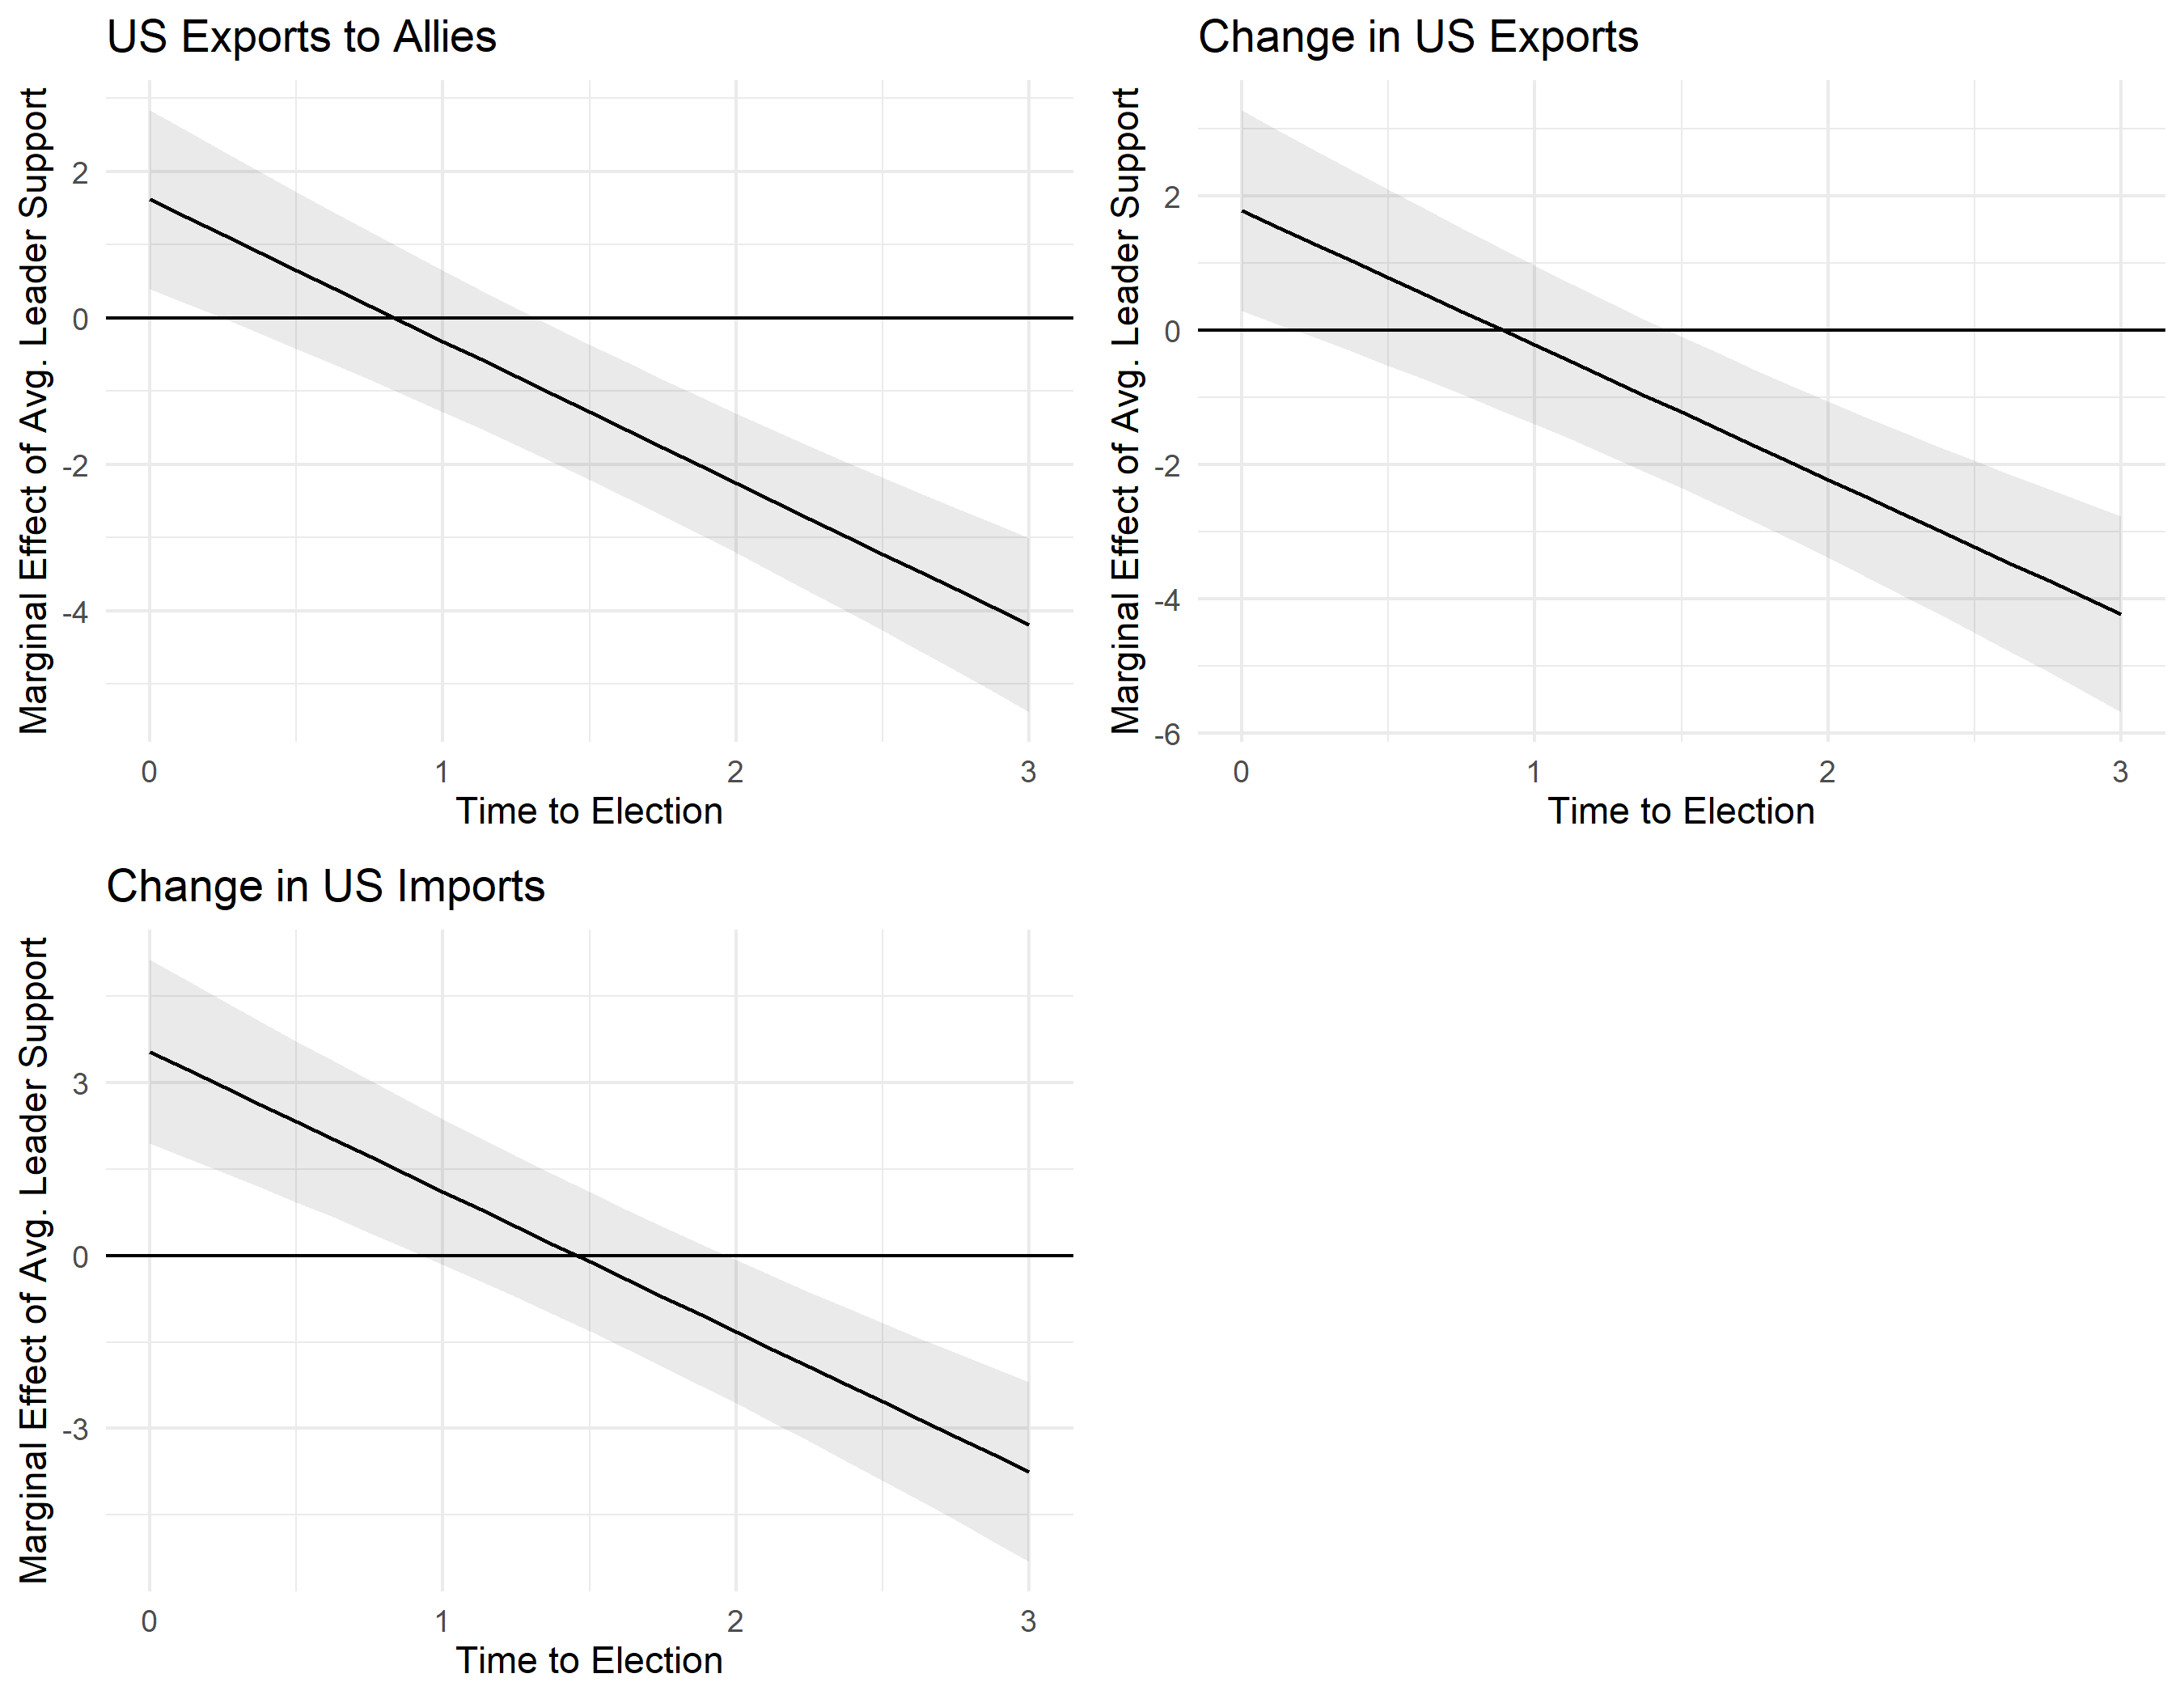
\includegraphics[width=0.95\textwidth]{../figures/me-plots-us.png}
	\caption{Estimated marginal effect of changes in signals of support by the incumbent leader trade between the United States and allied states, 1950 to 2010. The first model models annual major power exports and includes a lagged dependent variable. The second model regresses changes in exports on the explanatory variables. The third model examines changes and includes dyadic fixed effects. The fourth model assesses changes in imports. Points mark the coefficient estimate and error bars summarize the 95\% confidence interval.}
	\label{fig:me-plots-us}
\end{figure}


% control variables show other suggestive evidence of a cycle
Some of the other estimates in \autoref{tab:us-model-coefs} and \autoref{fig:me-plots-us} suggest an electoral cycle in U.S. trade with allies.
Overall trade, including both imports and exports, is higher when leaders offer more support early in their tenure.
Improved trade balances in election years are the result of larger decreases in imports than exports, though both trade flows are lower in election years.
Negative trade balances from leader support reflect greater increases in U.S. imports than U.S. exports. 


% improved trade balance
These results are consistent with the economic concessions hypothesis. 
When leaders have previously demonstrated commitment to their allies, those allies increase their imports in election years.
In the next analysis, I show that in the United State, these increases in exports are concentrated in electorally competitive states.



\section{Swing States and U.S. Exports to Allies in Election Years}


Greater U.S. exports to allied states during election years are partially a result of increased exports from swing states.
In election years, allied states import more goods than other states, and these imports are concentrated in important electoral states.
The result holds across two measures of electoral importance--- prior electoral competitiveness and pivot proximity \citep{Wright2009}.


To examine state trade, I fit a gravity model of trade to a dyadic dataset of logged exports from U.S. states to foreign countries during election years.
This analysis employs exports data from the St. Louis Federal Reserve and runs from 2002 to 2020.
The key independent variables are a dummy indicator of whether the destination country has a defense pact with the United States and two distinct measures of electoral competition. 
Because I expect that allies will be more likely to import from electorally competitive areas to maximize the impact of their economic concessions, allied imports from swing states should be higher than imports from other states in election years. 
The first electoral competition measure is the difference in the two-party vote share in the last presidential election.
Smaller differences in the vote share imply greater competition.
The second measure captures a state's pivot proximity in the election results. 
The pivot state is the state that, after ranking states by the vote share of the winner, gives them 270 electoral votes \citep{Wright2009}.
Keeping the same ordering, states are then close or far from the pivot. 
Pivot proximity thus encompasses vote share and electoral college considerations. 
Low pivot proximity scores implies a state was closer to providing the winning margin and was thus more important, while high proximity distance implies a state was unlikely to put the winning candidate over the top.\footnote{To maximize the number of elections in this analysis, I do not examine the conditioning effect of prior leader support, as the latent support measure only runs through 2010.} 


Because smaller pivot proximity and vote differences imply greater competition, I expect that the interaction of U.S. alliance and these variables will be negative. 
The U.S. alliance constituent term should be positive, as alliances support trade regardless of how pivotal a state may be \citep{GowaMansfield2004, Fordham2010}. 
I have no strong expectations about the electoral competition constituent term.


These models adjust for likely correlates of alliances, electoral competition and trade.
First, standard gravity model controls include the logged population and GDP of each state and corresponding country destination. 
I also adjust for the reelection years of George W. Bush, Barack Obama and Donald Trump with separate dummy indcators, as well as the exchange rate and government spending as a share of GDP in the destination state. 
A lagged dependent variable adjusts for temporal autocorrelation in dyadic exports.
To account for dyadic clustering, especially the diffusion of key electoral competition in a state across trading dyads with multiple partners, I employ a cluster-robust sandwich estimator for the standard errors \citep{Aronowetal2015}.



\subsection{Results}

As expected, allied states import more from U.S. states than other countries during election years. 
Crucial states in the electoral college export more to allies that other states. 
This is consistent with claims that allies make electorally strategic economic concessions. 


\autoref{fig:state-model-coefs} presents the coefficient estimates from the two primary regression models. 
The constituent term for the alliance variable is positive, which indicates that when vote difference is zero, or a state was pivotal in the Electoral College, allied states import more than other states. 
Among non-allied states, electoral salience does not have a clear association with exports. 
The negative interactions between alliances and electoral competition measures indicate that decreasing electoral salience reduces the association between an alliance and exports. 



\begin{figure}[htpb]
	\centering
		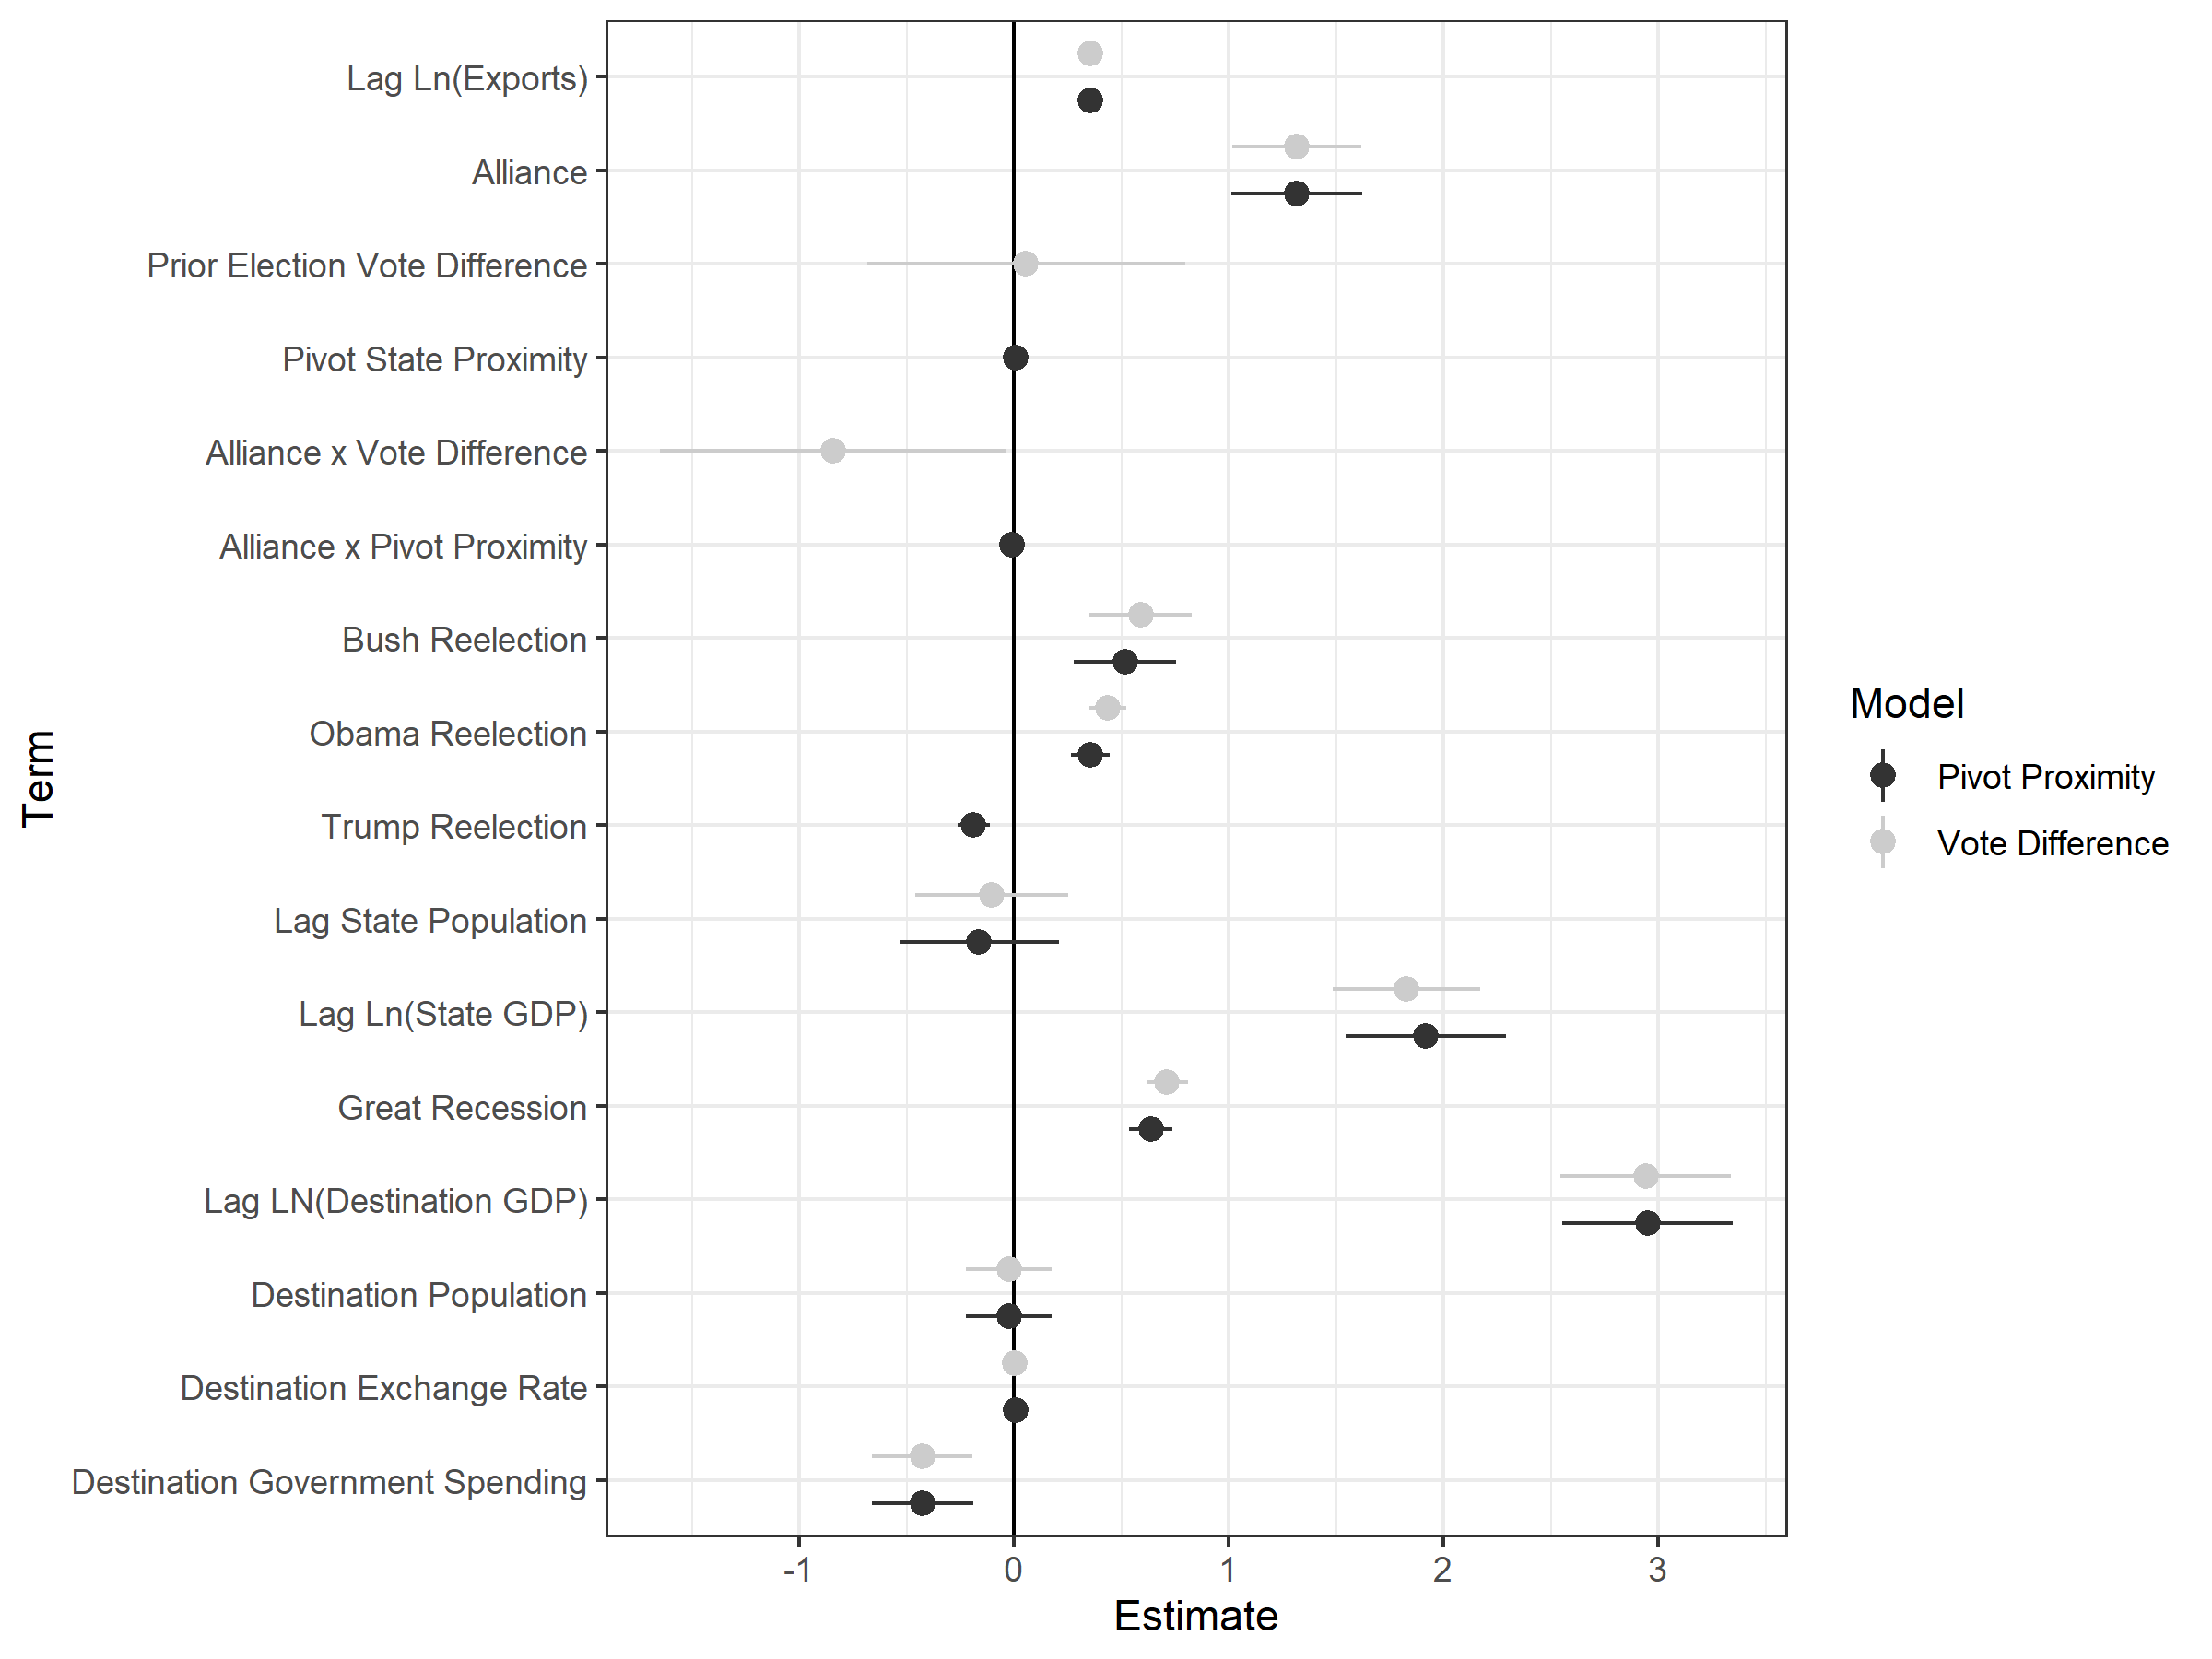
\includegraphics[width=0.95\textwidth]{../figures/state-model-coefs.png}
	\caption{Coefficient estimates from a gravity model of exports from U.S. states to foreign countries, 2002 to 2020. Points mark the coefficient estimates and error bars summarize 95\% confidence intervals.}
	\label{fig:state-model-coefs}
\end{figure}


The control variables in the model are also generally sensible. 
Increasing GDP in the state of origin and international destination both increase exports. 
Trump's reelection in 2020 is associated with far lower exports than other elections due to the Covid-19 pandemic. 


To show the interactions, \autoref{fig:me-all-state} presents the estimated marginal effect of an alliance on exports across the range of electoral competition. 
As prior election vote differences or proximity to the electoral pivot increase and electoral competition falls, allied states still import more than other states, but they import less, relative to more competitive states. 
This implies that allies have a slight preference for swing state exports during election years. 


\begin{figure}[htpb]
	\centering
		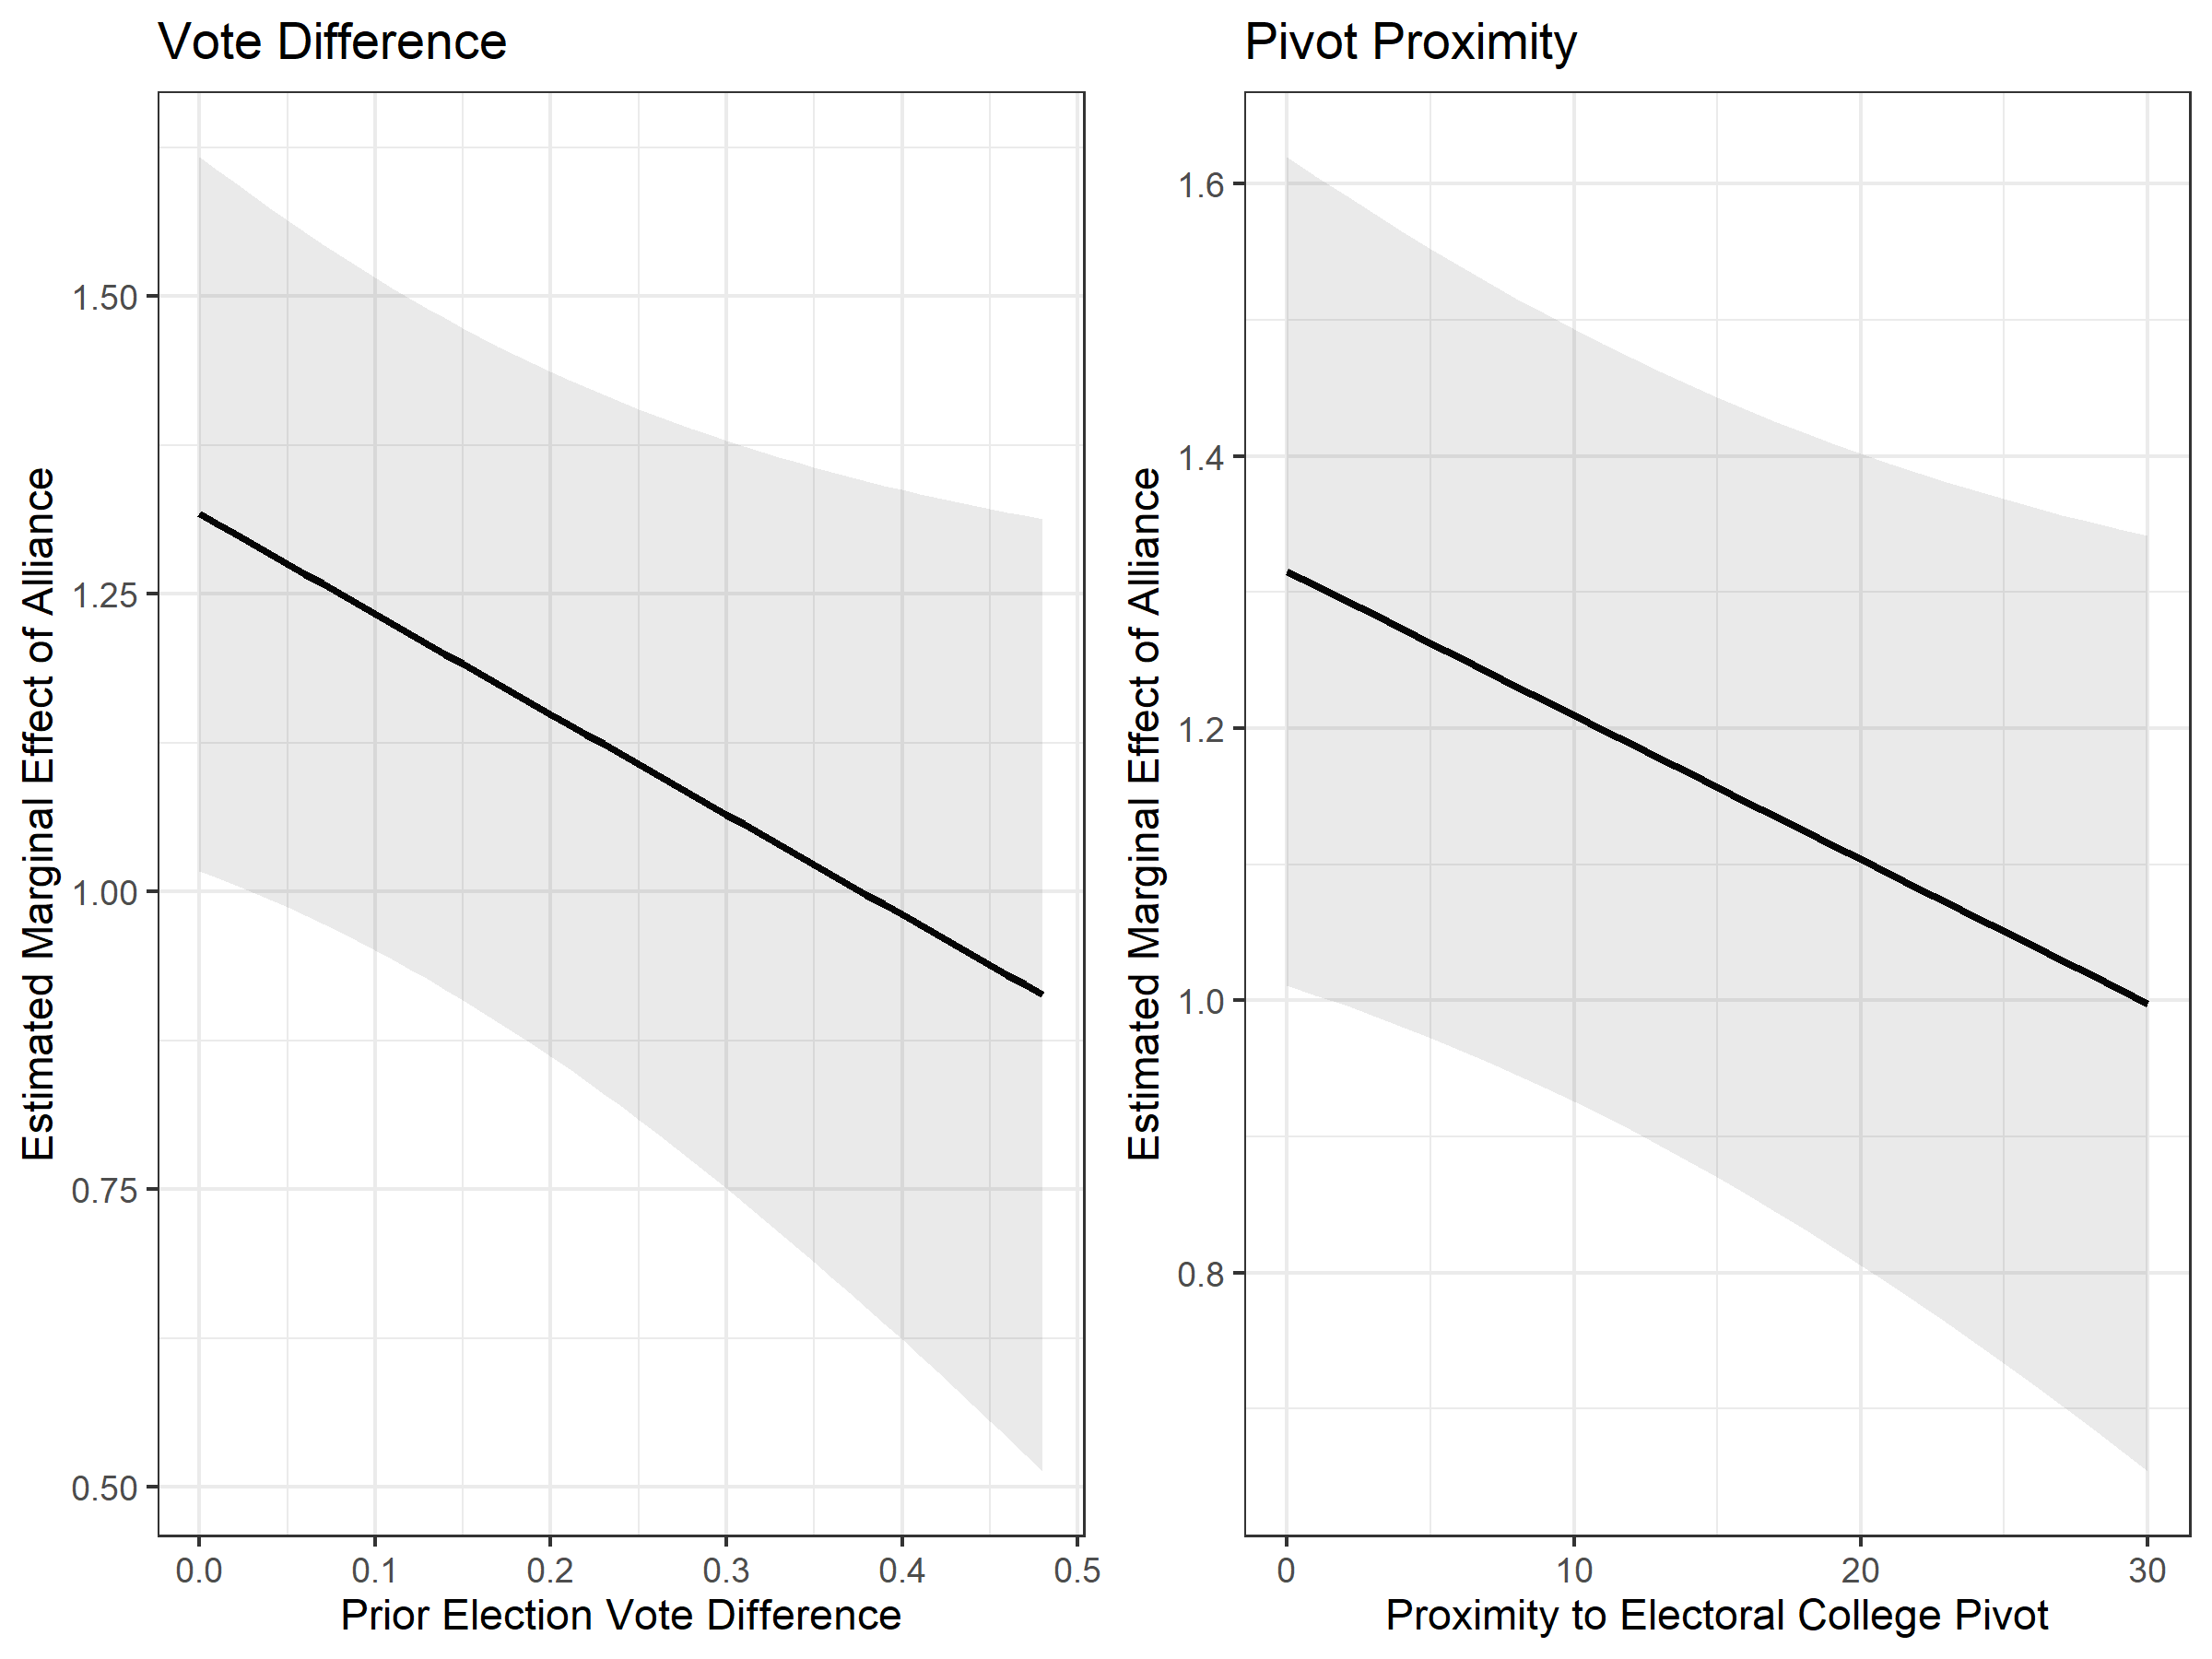
\includegraphics[width=0.95\textwidth]{../figures/me-all-state.png}
	\caption{Estimated marginal effect of an alliance on exports from U.S. states to foreign countries across two measures of electoral competitiveness, 2002 to 2020. Smaller vote difference or pivot proximity implies greater electoral competition.}
	\label{fig:me-all-state}
\end{figure}


This suggests that allied economic concessions in election years are targeted. 
U.S. allies concentrate their imports in states that are electorally crucial.
While this analysis does not show whether the export patterns are demand driven, where allies seek exports from competitive states, or supply driven as allies take on more goods from swing states where politicians want to bolster prosperity to win elections, allies help move trade flows for electoral advantage. 
As I show in the appendix, these interactions, as well as the conditional relationship between prior leader support and trade around elections, are robust to alternative specifications and functional forms \citep{Hainmuelleretal2019}.



\section{Allied Tariffs} 


The final analysis scrutinizes the claim that allies will be less likely to make structural trade concessions. 
I test this claim by modeling allied tariffs on U.S. goods with the same approach for testing the impact of prior leader support and elections. 
I find little evidence that increasing leader support reduces average allied tariffs or maximum tariff rates, even as proximity to elections increases. when tariffs are weighted by import volume. 


These models use tariff data from United Nations Conference on Trade and Development (UNCTAD)'s Trade Analysis and information systems (TRAINS) database. 
The tariff data starts in 1988 and limited temporal coverage in some control variables means that the analysis stops in 2010.\footnote{I include the European Union in the analysis because the EU is a key U.S. trade partner. I use with the average of presidential support in each year as the key independent variable.}
I analyze two outcome measures; average tariffs weighted by import volume and logged maximum tariffs. 
As in the analyses of exports and imports, I employ robust m-estimation with Tukey's biweight function because tariffs have substantial outliers.


% justify outcome measures
I use weighted average and maximum tariff rates to measure structural changes in allied trade policy because these measures capture crucial areas of domestic political competition.
Goods with greater U.S. exports are more salient to domestic industries. 
Maximum tariff rates likely reflect areas of particular political concern.


% summarize results
\autoref{tab:tariff-model-coefs} presents the estimates from robust regression models of weighted average allied tariffs and maximum tariff rates. 
There is less evidence that prior leader support reduces allied tariffs in the interaction coefficients. 
The average leader support constituent term is negative for weighted tariffs, but it is of small magnitude and uncertain direction.
Greater prior leader support increases maximum allied tariffs even in election years, however.
As is the case in other models, the years to election constituent term does not have a direct interpretation.
Both interaction terms are positive, though the direction of the maximum tariff interaction is unclear. 

% add table of coefficient estimates 
\begin{table}
\centering
\begin{table}
\centering
\begin{tabular}[t]{lcc}
\toprule
  & Allied Tariffs & Maximum Tariffs\\
\midrule
Avg Leader Support & -0.045 & 0.623\\
 & (-0.620, 0.530) & (0.439, 0.807)\\
Years to Election & -0.261 & -0.034\\
 & (-0.526, 0.004) & (-0.119, 0.051)\\
Years to Election x Avg Leader Support & 0.272 & 0.035\\
 & (0.027, 0.516) & (-0.043, 0.114)\\
Incumbent & 0.573 & -0.034\\
 & (-0.271, 1.417) & (-0.304, 0.237)\\
Allied Democracy & -1.506 & 0.900\\
 & (-2.085, -0.926) & (0.715, 1.086)\\
Change US GDP & 0.000 & 0.000\\
 & (0.000, 0.000) & (0.000, \vphantom{2} 0.000)\\
Change Ally GDP & 0.000 & 0.000\\
 & (0.000, 0.000) & (0.000, \vphantom{1} 0.000)\\
Pop. Weighted Distance & 0.000 & 0.000\\
 & (0.000, 0.000) & (0.000, 0.000)\\
Contiguous & -0.966 & 0.128\\
 & (-2.430, 0.497) & (-0.342, 0.597)\\
Common Language & 3.179 & -0.489\\
 & (2.534, 3.824) & (-0.696, -0.282)\\
Former Colony & -1.803 & 0.277\\
 & (-2.826, -0.779) & (-0.052, 0.605)\\
Ongoing MID & -1.490 & 1.678\\
 & (-3.544, 0.564) & (1.019, 2.336)\\
Shared IGOs & -0.142 & -0.003\\
 & (-0.175, -0.109) & (-0.014, 0.007)\\
Lag Ally Latency & 3.420 & 0.143\\
 & (2.482, 4.358) & (-0.158, 0.443)\\
Lag Rivalry & 0.697 & -0.397\\
 & (0.221, 1.172) & (-0.550, -0.245)\\
Prior Adversary Signal & -1.009 & 0.029\\
 & (-1.405, -0.614) & (-0.098, 0.156)\\
\midrule
N & 809 & 809\\
\bottomrule
\end{tabular}
	\caption{Coefficient estimates from models of allied tariffs on US exports, 1988 to 2010. The first model addresses each ally's annual average tariff on U.S. exports, weighted by import volume. The second model addresses the log maximum tariff rate. 95\% confidence intervals in parentheses.}
	\label{tab:tariff-model-coefs}
\end{table}

	\caption{Coefficient estimates from models of allied tariffs on US exports, 1988 to 2010. The first model addresses each ally's annual average tariff on U.S. exports, weighted by import volume. The second model addresses the log maximum tariff rate. 95\% confidence intervals in parentheses.}
	\label{tab:tariff-model-coefs}
\end{table}


\autoref{fig:tariff-me} presents how election proximity modifies the impact of leader support on allied tariff rates.
In election years, greater leader support has a substantively small but uncertain association with weighted average allied tariffs. 
The impact of support rises as time to an election increases, however. 
Early in presidential terms, signals of support for allies are associated with increased tariffs. 
Allies may avoid antagonizing friendly leaders with tariff increases around election years, but there is little evidence that they make structural trade changes.


\begin{figure}[htpb]
	\centering
		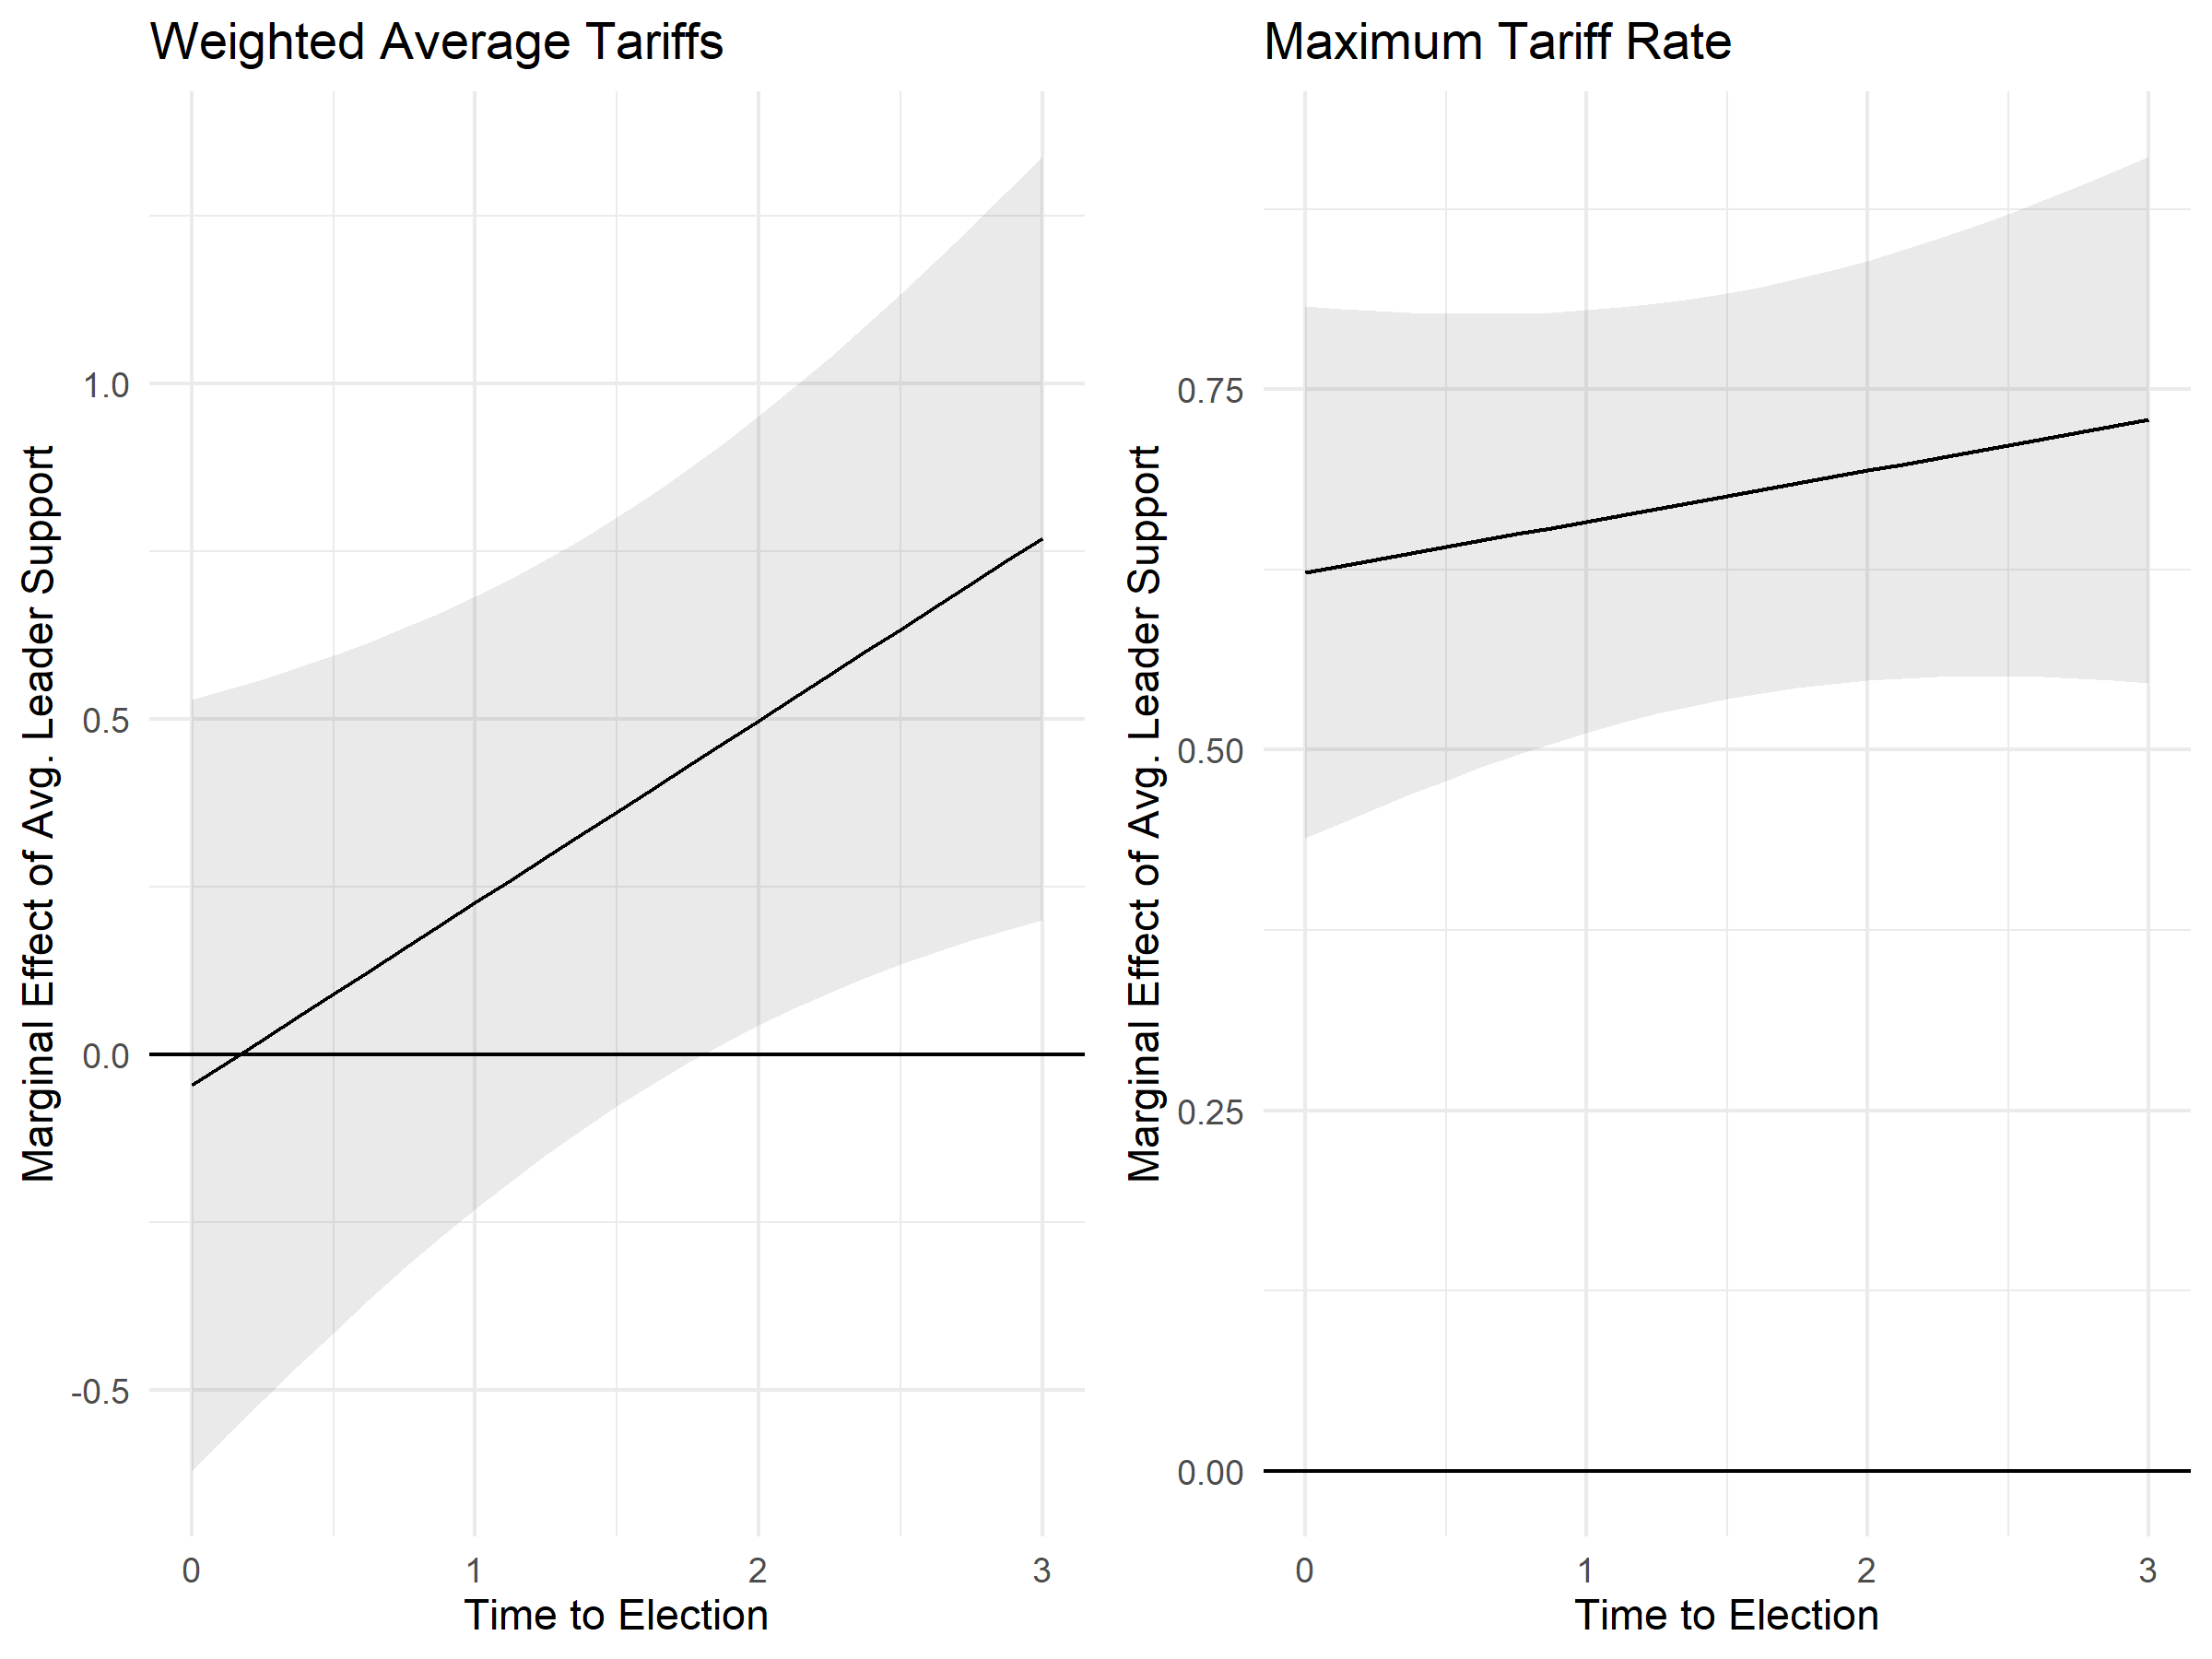
\includegraphics[width=0.95\textwidth]{../figures/tariff-me.png}
	\caption{Estimated marginal effect of of a two standard deviation increase in average signals of support by the incumbent leader on allied tariffs on U.S. exports, 1988 to 2010. The first model addresses each ally's annual average tariff on U.S. exports, weighted by import volume. The second model examines the log maximum tariff rate.}
	\label{fig:tariff-me}
\end{figure}


Maximum tariffs respond to commitment signals, and this relationship does not fluctuate with U.S. electoral cycles.
When leaders reassure their allies at any point in their tenure, allied states increase their maximum tariff on U.S. goods.
Thus, allies take advantage of greater confidence in U.S. commitment to increase protection for crucial domestic interests.


Therefore, the balance of evidence suggests that allied states do not reduce their tariffs to help supportive leaders win election.
Allied trade concessions are temporary, rather than structural.
Commitment signaling is more likely to increase allied trade barriers.
Reduced commitment might lower allied tariffs, albeit at the cost of allied trade support in election years.


\newpage
\singlespace
 
\bibliography{../../MasterBibliography} 


\end{document}